\chapter{ကားရဲလ်နှင့် ကွန်ထရိုးလ် စတိတ်မန့်များ}\label{ch:ch02}


ကားရဲလ်ပရိုဂရမ်တစ်ခု ဖွဲ့စည်းတည်ဆောက်ပုံကို ရှေ့အခန်းမှာ လေ့လာခဲ့ကြပြီး ကွန်ထရိုးလ် စတိတ်မန့်တွေ ဖြစ်ကြတဲ့ \fCodeBf{for} \fEn{loop}\fEn{,} \fCode{while} \fEn{loop}\fEn{,} \fCodeBf{if} နဲ့ \fCodeBf{if}\fCode{...}\fCodeBf{else} တို့ကို အခုဆက်လက် လေ့လာကြပါမယ်။ ပရိုဂရမ်တစ်ခုကို \fEn{run} တဲ့အခါ ပရိုဂရမ်ကုဒ်ထဲက ညွှန်ကြားချက်တွေအတိုင်း ကွန်ပျူတာက လုပ်ဆောင်ပေးတာပါ။ ဒီလိုလုပ်ဆောင်ပေးတာကို အက္ခစီကျူ့ \fEn{(execute)} လုပ်တယ်လို့ ခေါ်တယ်။ ကွန်ထရိုးလ်စတိတ်မန့်တွေဟာ ပရိုဂရမ်တစ်ခုရဲ့ \fEn{execution flow} ကို ထိန်းချုပ်ပေးတာ ဖြစ်တဲ့အတွက် \fEnEmp{control flow statements} တွေလို့လည်း ခေါ်ပါတယ်။

\section{\fSecCodeBf{for} loop}
% ============================

ကွန်ထရိုးလ်စတိတ်မန့် တစ်မျိုးဖြစ်တဲ့ \fCodeBf{for} \fEn{loop} ဟာ စတိတ်မန့် တစ်ခု (သို့) စတိတ်မန့် တစ်စုကို သတ်မှတ်ထားတဲ့ အကြိမ်အရေအတွက် ပြည့်အောင် ထပ်ခါထပ်ခါ ပြန်ကျော့ပေးပါတယ်။  \fCode{move} ကို နှစ်ဆယ့်ငါးကြိမ် ကျော့ပေးဖို့ \fCode{for} \fEn{loop} နဲ့ အခုလို 
%
\setlength{\fboxsep}{0pt}
\begin{minted}[frame=\mintframe, framerule=\mintrule,framesep= \mintsep, xleftmargin=\xlftmargin
    , bgcolor=mintbgcolor,rulecolor=mintrulecolor
    , python3=true,escapeinside=ßß]{python}
for i in range(25):
    move()
\end{minted}
%
ရေးရပါတယ်။ \fCode{put\_beeper}\fEn{,} \fCode{move}\fEn{,} \fCode{turn\_left} စတိတ်မန့် သုံးကြောင်းတစ်စုကို အကြိမ်တစ်ရာ ကျော့ချင်ရင် ဒီလိုပါ 
%
\setlength{\fboxsep}{0pt}
\begin{minted}[frame=\mintframe, framerule=\mintrule,framesep= \mintsep, xleftmargin=\xlftmargin
    , bgcolor=mintbgcolor,rulecolor=mintrulecolor
    , python3=true,escapeinside=ßß]{python}
for i in range(100):
    put_beeper()
    move()
    turn_left()
\end{minted}
%

နှစ်ဆယ့်ငါးကြိမ်ကို \fCode{range(25)}\fEn{,} အကြိမ်တစ်ရာကို \fCode{range(100)} စသည်ဖြင့် တွေ့ရတယ်။ ယေဘု\allowbreak ယျအားဖြင့် အကြိမ်အရေအတွက် \fEnEmp{N} ကြိမ် ကျော့ချင်ရင်  
%
\setlength{\fboxsep}{0pt}
\begin{minted}[frame=\mintframe, framerule=\mintrule,framesep= \mintsep, xleftmargin=\xlftmargin
    , bgcolor=mintbgcolor,rulecolor=mintrulecolor
    , python3=true,escapeinside=ßß]{python}
for ß$x$ß in range(ß$N$ß):
    ß$statement_1$ß
    ß$statement_2$ß
    ß$statement_3$ \fEn{etc.}ß
\end{minted}
%
ပုံစံနဲ့ သတ်မှတ်ရတာ။ \fEnEmp{N} က  အကြိမ်အရေအတွက်ကို ဖော်ပြတဲ့ ကိန်းပြည့်ဂဏန်းဖြစ်တယ်။ \fCode{for} \fEn{loop} ရေးတဲ့အခါ ကော်လံ \fCode{:} မကျန်ခဲ့ဖို့ သတိပြုရပါမယ်။ $x$ ဟာ ဗေရီရေဘဲလ်တစ်ခုဖြစ်ပြီး \fCode{i}\fEn{,} \fCode{j}\fEn{,} \fCode{k} စတဲ့ အက္ခရာတစ်ခုနဲ့ ကိုယ်စားပြုလေ့ရှိတယ်။

\begin{mytcbox}
ပြန်ကျော့စေချင်တဲ့ စတိတ်မန့်တွေကို \fCode{for} ရဲ့ ညာဘက်ကို အင်ဒန့်ထ် လုပ်ပေးရပါမယ်။ အောက်ပါအတိုင်းဆိုရင် \fCode{put\_beeper} ကိုပဲ အကြိမ်တစ်ရာ လုပ်မှာပါ။ \fCode{move} နဲ့ \fCode{turn\_left} ပြန်ကျော့မဲ့ထဲမှာ မပါတော့ဘူး။
\setlength{\fboxsep}{0pt}
\begin{minted}[frame=\mintframe, framerule=\mintrule,framesep= \mintsep, xleftmargin=\xlftmargin
    , bgcolor=boxfillcolor,rulecolor=mintrulecolor
    , python3=true,escapeinside=ßß]{python}
for i in range(100):
    put_beeper()
move()
turn_left()
\end{minted}
\end{mytcbox}

%
\begin{figure}[tbh!]
\begin{tikzpicture}
    \node[anchor=south west,inner sep=0] (image) at (0,0)
        {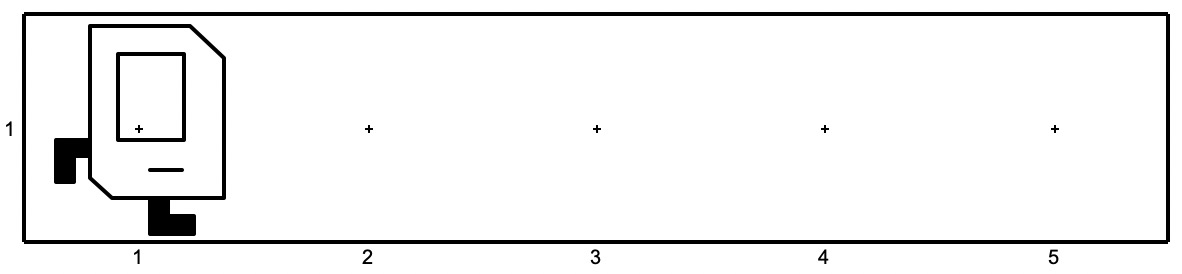
\includegraphics[scale=0.2, trim={2.4mm 2mm 2mm 2mm},clip]{images/ch02/mrofb/before.jpg}};
\end{tikzpicture}
\caption{} 
\label{fig:mrofb-bef}
\end{figure}
%
ပုံ (\fRefNo{\ref{fig:mrofb-bef}}) ကားရဲလ်ကမ္ဘာမှာ ကွန်နာအားလုံးမှာ ဘိပါတစ်ခုစီ ချထားပေးရမယ်။ ကွန်နာငါးခုရှိတာမို့လို့ စုစုပေါင်း ဘိပါငါးခု ချထားရမှာပါ။ \fCode{move} ကတော့ လေးကြိမ်ပဲ လုပ်ရမယ် (ကားရဲလ်ရှေ့မှာ ကွန်နာလေးခုပဲ ရှိတယ်)။ ဒီအတွက်ကို အခုလိုရေးနိုင်ပါတယ်။
%
\setlength{\fboxsep}{0pt}
\begin{minted}[frame=\mintframe, framerule=\mintrule,framesep= \mintsep, xleftmargin=\xlftmargin
    , bgcolor=mintbgcolor,rulecolor=mintrulecolor
    , python3=true,escapeinside=ßß]{python}
# File: make_row_of_5_beepers.py
from stanfordkarel import *


def main():
    for i in range(4):
        put_beeper()
        move()

    put_beeper()


if __name__ == "__main__":
    run_karel_program("make_row_of_5_beepers")

\end{minted}
%

\fCode{for} \fEn{loop} ဟာ \fCode{put\_beeper} နဲ့ \fCode{move} ကို လေးကြိမ်ကျော့ပေးမှာပါ။ တစ်ကြိမ်ပြီးတိုင်း ရှိနေမဲ့ အနေအထား တစ်ခုချင်းစီကို ပုံ (\fRefNo{\ref{fig:mrofb_iters}})  မှာ တွေ့နိုင်ပါတယ်။ လေးကြိမ်မြောက် နောက်ဆုံးတစ်ကျော့အပြီး ပုံ (\fRefNo{\ref{fig:mrofb_iters}}) (င) မှာ ဘိပါတစ်ခုလိုနေသေးတာ တွေ့ရမယ်။ \fCode{for} \fEn{loop} ပြီးတဲ့အခါ \fCode{put\_beeper} တစ်ခါထပ်လုပ်ပေးတော့မှ တစ်တန်းလုံးအပြည့်ဖြစ်သွားမှာပါ။


\begin{figure}[thb!]
    \newcommand{\figpctw}{0.49}
    \begin{subfigure}[t]{{\figpctw}\textwidth}
        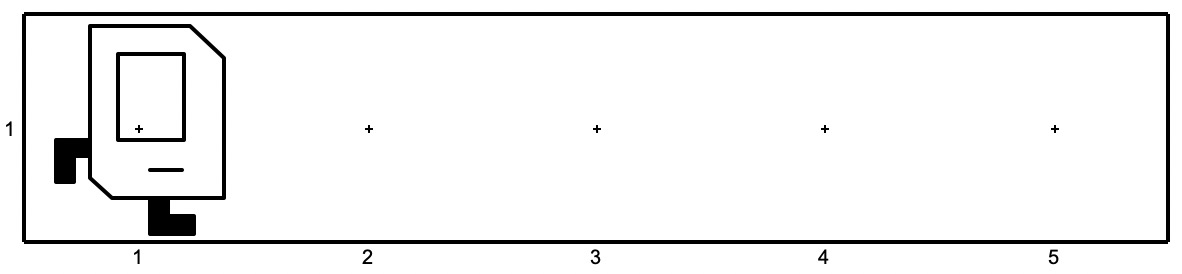
\includegraphics[scale=0.15]{images/ch02/mrofb/before.jpg}
        \caption{မူလ အနေအထား}    
    \end{subfigure}
    \begin{subfigure}[t]{{\figpctw}\textwidth}
        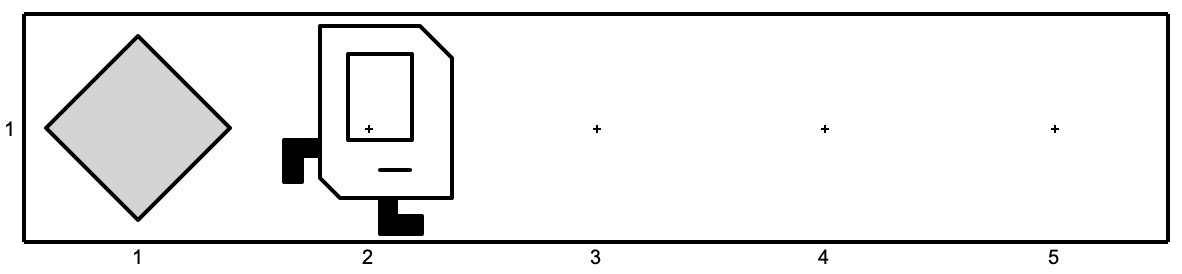
\includegraphics[scale=0.15]{images/ch02/mrofb/1st_iter.jpg}
        \caption{ပထမ တစ်ကျော့ပြီး}    
    \end{subfigure}
    \begin{subfigure}[t]{{\figpctw}\textwidth}
        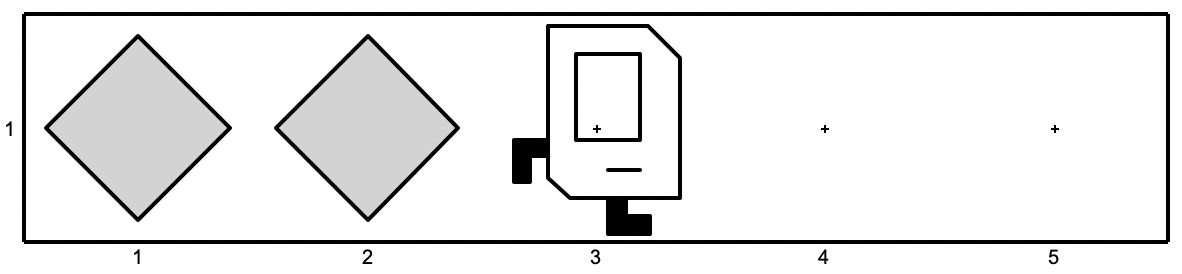
\includegraphics[scale=0.15]{images/ch02/mrofb/2nd_iter.jpg}
        \caption{ဒုတိယ တစ်ကျော့ပြီး}    
    \end{subfigure}
    \begin{subfigure}[t]{{\figpctw}\textwidth}
        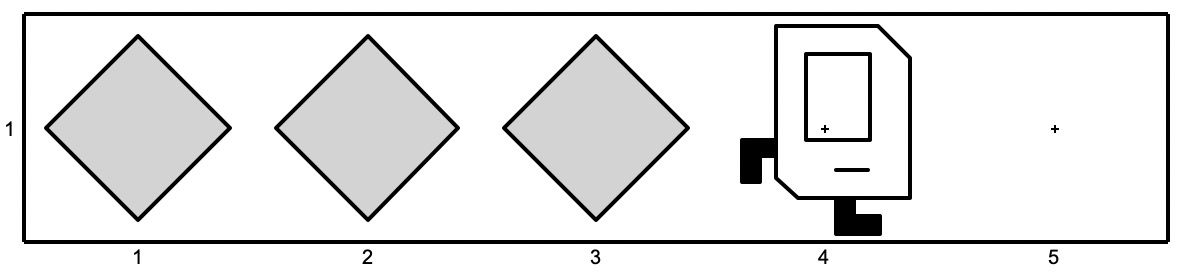
\includegraphics[scale=0.15]{images/ch02/mrofb/3rd_iter.jpg}
        \caption{တတိယ တစ်ကျော့ပြီး}    
    \end{subfigure}
    \begin{subfigure}[t]{{\figpctw}\textwidth}
        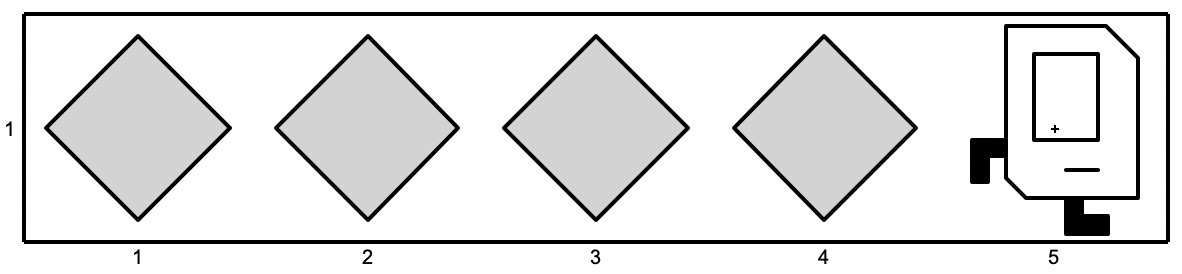
\includegraphics[scale=0.15]{images/ch02/mrofb/4th_iter.jpg}
        \caption{စတုတ္ထမြောက် ကျော့ပြီး}    
    \end{subfigure}
    \begin{subfigure}[t]{{\figpctw}\textwidth}
        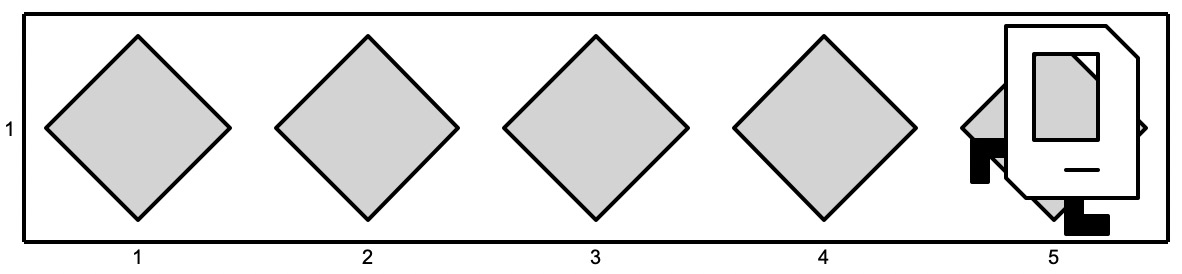
\includegraphics[scale=0.15]{images/ch02/mrofb/after.jpg}
        \caption{နောက်ဆုံး \fCptCodeBf{putBeeper} လုပ်ပြီး}    
    \end{subfigure}
    \caption{}
    \label{fig:mrofb_iters}
\end{figure}

\subsection*{Off-by-one bug}

ပြီးခဲ့တဲ့ဥပမာမှာ \fCode{for} \fEn{loop} အပြီး \fCode{put\_beeper} မလုပ်မိရင် ပရိုဂရမ်ဟာ လိုချင်တဲ့အတိုင်း မဖြစ်ပါဘူး။  ဘိပါတစ်ခုလိုနေမယ်။ ဒီလိုပြဿနာမျိုးဟာ အဖြစ်များတဲ့ အမှားဖြစ်ပြီး \fEnEmp{off-by-one bug} လို့ခေါ်ပါတယ်။ \fEn{Loop} သုံးတဲ့အခါ ကြုံရလေ့ရှိတဲ့ ဖြစ်တတ်တဲ့ အမှား \fEn{(\textit{bug})} ဖြစ်တယ်။ သတ်မှတ်ထားတဲ့အတိုင်း၊ ဖြစ်သင့်တဲ့အတိုင်း ပရိုဂရမ်က အလုပ်မလုပ်ဘဲ ဖြစ်နေတဲ့ အမှားကို ကွန်ပျူတာအသုံးအနှုန်းမှာ \fEn{bug} လို့ခေါ်တာပါ။ \fEn{Bug} ကိုလိုက်ရှာပြီး မှန်အောင်ပြင်ပေးတာကိုတော့ \fEn{debug} လုပ်တယ်လို့ခေါ်ပါတယ်။

ဘိပါတစ်ခုကျန်ခဲ့တဲ့ အမှားမျိုးဟာ \fEn{off-by-one bug} သာဓကတစ်ခုမျှသာ ဖြစ်တယ်။ ခုနှစ်နဲ့ ဆယ့်သုံးကြား ဂဏန်း ခုနှစ်လုံးရှိပါတယ် (ခုနှစ်နဲ့ ဆယ့်သုံးအပါဝင် ဆိုလျှင်)။  \(13 - 7 = 6\) လို့တွက်မိရင် တစ်လုံး လိုနေပါလိမ့်မယ်။ သုံးပေခြား တစ်တိုင် အလျားပေသုံးဆယ်ရှိ တဖြောင့်တည်း ခြံစည်းရိုးတစ်ခုအတွက် တိုင်စုစုပေါင်း တစ်ဆယ့်တစ်တိုင် လိုပါမယ်။ \(30 \div 3 = 10\) လို့ တွက်ရင် မမှန်ပါဘူး။ တစ်ခုလိုတာ အပြင် တစ်ခုပိုနေတာလည်း ဖြစ်တတ်တယ်။ စောနက ခြံစည်းရိုးမှာပဲ ထရံအချပ်အရေအတွက်ကတော့ ကိုးချပ်ဖြစ်ရမှာပါ။ \(30 \div 3 = 10\) လို့ တွက်ရင် တစ်ခုပိုနေပါမယ်။ ခုနှစ်နဲ့ ဆယ့်သုံးကို ထည့်မစဉ်းစားရင် ကြားမှာ ဂဏန်းငါးလုံးရှိတာပါ။ \(13 - 7 = 6\) လို့တွက်မိရင် တစ်လုံး ပိုနေပါလိမ့်မယ်။ ဒီ ဥပမာ အားလုံးဟာ အခြေခံသဘောတရားအားဖြင့် သိပ်မကွာခြားတဲ့ \fEn{off-by-one bug} ပုံစံကွဲအမျိုးမျိုး ဖြစ်တယ်။

\subsection*{‘Make Row of Five Beepers’ ဒုတိယ ဗားရှင်း}
ပရိုဂရမ်ရေးတဲ့အခါ ပရိုဂရမ်မာတွေ တစ်ယောက်နဲ့တစ်ယောက် စဉ်းစားပုံ စဉ်းစားနည်း၊ ဖြေရှင်းနည်း ထပ်တူကျလေ့မရှိပါဘူး။ ဘိပါငါးခု အတန်းလိုက် ချပေးတဲ့ ပရိုဂရမ်ကိုပဲ နောက်ဗားရှင်းတစ်မျိုးနဲ့ ရေးနိုင်ပါတယ်။
%
\setlength{\fboxsep}{0pt}
\begin{minted}[frame=\mintframe, framerule=\mintrule,framesep= \mintsep, xleftmargin=\xlftmargin
    , bgcolor=mintbgcolor,rulecolor=mintrulecolor
    , python3=true,escapeinside=ßß]{python}
def main():
    put_beeper()
    for i in range(4):
        move()
        put_beeper()
\end{minted}
%
\fCode{for} \fEn{loop} မစခင် \fCode{put\_beeper} လုပ်ထားတာ၊ \fCode{move} နဲ့ \fCode{put\_beeper} အစဉ်ပြောင်းသွားတာ (ပထမ ဗားရှင်းနဲ့ ပြောင်းပြန်ဖြစ်နေတာ) သတိထားကြည့်ပါ။

\section{အင်ဒန့်ထ်လုပ်ခြင်းနှင့် ကုဒ်စထရက်ချာ}

\fEn{Python} ဟာ အင်ဒန့်ထ်လုပ်ခြင်းဖြင့် ပရိုဂရမ်ကုဒ် ဖွဲ့စည်းပုံ စထရက်ချာကို ဖော်ပြတဲ့ \fEn{programming language} ဖြစ်ပါတယ်။ \fEn{Python} ကုဒ်တွေကို ဘလောက် \fEn{(\textit{block})} တွေနဲ့ ဖွဲစည်းထားတယ်လို့ ရှုမြင်နိုင်တယ်။ ဘလောက်ဆိုတာ ကုဒ်တွေကို အုပ်စုတစ်စု အဖြစ် ဖွဲ့စည်းထားတာကို ဆိုလိုတာပါ။ 
%
\setlength{\fboxsep}{0pt}
\begin{minted}[frame=\mintframe, framerule=\mintrule,framesep= \mintsep, xleftmargin=\xlftmargin
    , bgcolor=mintbgcolor,rulecolor=mintrulecolor
    , python3=true,escapeinside=ßß]{python}
def main():
    put_beeper()
    for i in range(4):
        move()
        put_beeper()
    pick_beeper()
turn_left()
\end{minted}
%
အခု \fEn{Python} ကုဒ်မှာ အင်ဒန့်ထ်မလုပ်ထားဘဲ  ဘယ်ဘက်စွန်း ကပ်ရေးထားတဲ့ \fCode{\textbf{def} main():} (ဖန်ရှင်ခေါင်းစည်း) ဟာ အပေါ်ဆုံးအဆင့် \fEn{(top level)} ဖြစ်တယ်လို့ ယူဆတယ်။ ဖန်ရှင်ခေါင်းစည်းအောက် အင်ဒန့်ထ်လုပ်ထားတဲ့ ကုဒ်လိုင်းအားလုံးဟာ \fCode{main} ဖန်ရှင် ဘလောက်ထဲမှာ အကျုံးဝင်တယ်။ \fCode{pick\_bee\allowbreak per} အထိပါတယ်။ \fCode{put\_beeper} (ပထမတစ်ခု)၊ \fCode{for} \fEn{loop} နဲ့ \fCode{pick\_beeper} တို့ဟာ ပထမအဆင့် အင်ဒန့်ထ်ဖြစ်တယ်။ 

တစ်ခါ \fCode{for} အောက်မှာ ဒုတိယတစ်ဆင့် အင်ဒန့်ထ်လုပ်ထားတဲ့ ကုဒ်လိုင်းအားလုံး \fCode{for} ဘလောက်ထဲမှာ အကျုံး\allowbreak ဝင်တယ်။ \fCode{move} နဲ့ \fCode{put\_beeper} ပါဝင်တယ်။ \fCode{pick\_beeper} ကတော့ ပထမအဆင့် ပြန်ဖြစ်သွားတဲ့အတွက် \fCode{for} ဘလောက်ထဲမှာမပါဘူး။ 

အောက်ဆုံး \fCode{turn\_\allowbreak left()} ကလည်း အင်ဒန့်ထ်လုပ် မထားတဲ့အတွက် အပေါ်ဆုံးအဆင့်ပဲ။ \fCode{\textbf{def} main():} နဲ့ အဆင့်တူတာပေါ့။ \fCode{main} ဖန်ရှင်ဘလောက် အပြင်ဘက်မှာလို့ ယူဆရမယ်။ 

အင်ဒန့်ထ်လုပ်ထားတဲ့ အဆင့်ကို ကြည့်ပြီး ဘလောက်တွေရဲ့ ဖွဲ့စည်းပုံကို ကွက်ကွက်ကွင်းကွင်း ထင်းကနဲ မြင်နိုင်တယ်။ အပေါ်ကကုဒ်ကို ကြည့်တာနဲ့ \fCode{main} ဖန်ရှင်ထဲမှာ \fCode{for} \fEn{loop} ရှိတယ်၊ \fCode{for} \fEn{loop} ထဲမှာ \fCode{move} နဲ့ \fCode{put\_beeper} ပါဝင်တယ်ဆိုတာ သိသာတယ်။ \fCode{pick\_beeper} ဟာ \fCode{for} \fEn{loop} အပြင်မှာ၊ \fCode{turn\_left} ဟာ \fCode{main} အပြင်မှာ ဆိုတာကို အင်ဒန့်ထ်လုပ်ထားတဲ့ အဆင့်က ဖော်ပြနေတယ်။





%အင်ဒန့်ထ်လုပ်ထားတဲ့ အဆင့်အရကြည့်ရင် \fCode{\textbf{def} main():} နဲ့ \fCode{turn\_left} က အဆင့်တူတယ်။ 

\section{\fSecCodeBf{while} loop}
အခြေအနေတစ်ရပ် မှန်နေသ၍ စတိတ်မန့်တွေကို တစ်ကြိမ်ပြီးတစ်ကြိမ် ပြန်ကျော့ လုပ်ဆောင်စေချင်ရင် \fCodeBf{while} \fEn{loop} ကို အသုံးပြုပါတယ်။  \fCode{for} နဲ့ \fCode{while} \fEn{loop} နှစ်ခုလုံးက ပြန်ကျော့ပေးတာ ဖြစ်ပေမဲ့ \fCode{for} ကို အကြိမ်အရေအတွက် အတိအကျသိတဲ့ကိစ္စမျိုးမှာ သုံးလေ့ရှိပြီး \fCode{while} ကိုတော့ ဘယ်နှစ်ကြိမ်လဲ ကြိုတွက်လို့မရဘဲ အခြေအနေ အပေါ်မူတည်ပြီး လုပ်ဆောင်ပေးရမဲ့ အကြိမ်အရေအတွက် ကွာခြားနိုင်တဲ့ ကိစ္စမျိုးတွေမှာ သုံးလေ့ရှိတယ်။ ဥပမာတစ်ခုနဲ့ ကြည့်ရင် ပိုနားလည်ပါလိမ့်မယ်။

(၁) လမ်းပေါ်မှာ ဘိပါတစ်ခုရှိမယ်။ ဘိပါ ဘယ်ကွန်နာမှာရှိမှာလဲ၊ လမ်းဘယ်လောက်အရှည်ဖြစ်မလဲ ကြိုတင်မသိဘူးလို့ ယူဆပါ။ နမူနာကမ္ဘာ တစ်ခုကို ပုံ (\fRefNo{\ref{fig:gpb1}}) မှာ တွေ့နိုင်တယ်။ ဘိပါကို သွားပြီး ကောက်ခိုင်းရပါမယ်။ အလားတူ မည်သည့်ကမ္ဘာအတွက်မဆို ဘိပါကောက်ပေးနိုင်ရမှာ ဖြစ်တယ်။
%
\begin{figure}[thb!]
    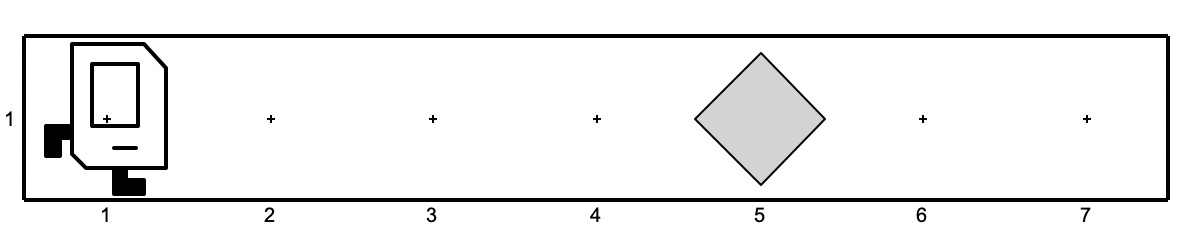
\includegraphics[width=0.8\textwidth]{images/ch02/gpb/at_fifth.jpg}
    \caption{}\label{fig:gpb1}
\end{figure}
%
ဘိပါရှိမဲ့ကွန်နာကို ကြိုတင်မသိထားတဲ့အတွက် ဘယ်နှစ်ကြိမ် \fCode{move} လုပ်ခိုင်းရမှာလဲ မသိဖြစ်နေတယ်။ အကြိမ်အရေအတွက် မသိတဲ့အတွက် \fCode{for} \fEn{loop} နဲ့ အဆင်မပြေတော့ပါဘူး။

ဘိပါမရှိသ၍ တစ်ကြိမ်ပြီးတစ်ကြိမ် \fCode{move} လုပ်ခိုင်းမယ်ဆိုရင် နောက်ဆုံးမှာ ဘိပါရှိတဲ့ကွန်နာကို ရောက်သွားမှာ သေချာပါတယ်။ အဲဒီလို လုပ်ခိုင်းဖို့ရာအတွက် \fCode{while} \fEn{loop} နဲ့ ရေးထားတာကို အခုလိုတွေ့ရပါမယ်။
%
\setlength{\fboxsep}{0pt}
\begin{minted}[frame=\mintframe, framerule=\mintrule,framesep= \mintsep, xleftmargin=\xlftmargin
    , bgcolor=mintbgcolor,rulecolor=mintrulecolor
    , python3=true,escapeinside=ßß]{python}
while no_beepers_present():
    move()
\end{minted}
%

ကားရဲလ်ဟာ အခြေခံကွန်မန်း လေးခုအပြင် လက်ရှိ ကွန်နာမှာ ဘိပါရှိ/မရှိ၊ ရှေ့မှာ နံရံပိတ်နေ/မနေ၊ အရှေ့ဘက်ကို မျက်နှာမူထား/မထား စတဲ့ သူနဲ့ (သို့) သူ့ရဲ့ကမ္ဘာနဲ့ သက်ဆိုင်တဲ့ အခြေအနေတစ်ရပ်ရပ် မှန်/မမှန် စစ်နိုင်ပါတယ်။ \fCode{no\_beepers\_present} က လက်ရှိ သူရှိနေတဲ့ ကွန်နာမှာ ‘ဘိပါ မရှိဘူးလား’ ဆိုတဲ့ အခြေအနေ စစ်ခိုင်းတာပါ။ လက်ရှိကွန်နာမှာ ဘိပါ ‘မရှိ’ ရင် ဒီအခြေအနေက မှန်တယ်လို့ ယူဆရမှာပေါ့။ အကယ်၍ ‘ရှိ’ နေရင်တော့ မှားတယ်လို့ ယူဆရမယ်။ အမှန် (သို့) အမှား ရလဒ်ထွက်မဲ့ ဒီလိုမျိုး အခြေအနေစစ် ကွန်မန်းတွေကို  ကွန်ဒီရှင် \fEn{(condition)} လို့ခေါ်ပါတယ်။

\fCode{while} \fEn{loop} အလုပ်လုပ်ပုံက ဒီလိုပါ။ \fCode{no\_beepers\_present} ကွန်ဒီရှင် စစ်ပါတယ်။ မှန်ရင်  \fCode{move} လုပ်ပါတယ်။ ပြီးရင် ကွန်ဒီရှင်ပြန်စစ်တယ်။ မှန်ရင် \fCode{move} ကို နောက်ထပ်တစ်ကြိမ် ထပ်ကျော့ပါတယ်။ ကွန်ဒီရှင်စစ်လိုက်၊ မှန်ရင် တစ်ခါထပ်ကျော့လိုက်၊ ကွန်ဒီရှင်ပြန်စစ်လိုက်၊ မှန်ရင် နောက်တစ်ခါထပ်ကျော့လိုက်၊ \fCode{...} ဒီအတိုင်းဆက်ပြီး ကွန်ဒီရှင်မှန်နေသ၍ \fCode{while} \fEn{loop} က \fCode{move} ကို ပြန်ကျော့ပေးမှာပါ။ ကွန်ဒီရှင် စစ်လိုက်လို့ မှားသွားပြီဆိုရင်တော့ ထပ်မကျော့တော့ဘဲ ရပ်သွားမှာဖြစ်တယ်။  \fCode{while} \fEn{loop} တစ်ကြိမ်ကျော့ပြီးတိုင်း ရှိနေမဲ့ အနေအထား တစ်ခုချင်းကို ပုံ (\fRefNo{\ref{fig:gpb_iters}})  မှာ  လေ့လာကြည့်ပါ။ လေးကြိမ်မြောက် ကျော့ပြီးနောက်  ကွန်ဒီရှင်စစ်လိုက်တဲ့အခါ မှားနေပြီ။ ဒီအခါ  \fCode{while} \fEn{loop} က ထပ်မကျော့တော့ဘူး။ ဒီလို \fEn{loop} က ပြန်ကျော့နေတာ ရပ်သွားရင် \fEn{loop} ကနေ ထွက်တယ် \fEn{(loop exits)} လို့ ပြောလေ့ရှိတယ်။ 

\begin{figure}[tb!]
    \hfuzz=100pt
    \newcommand{\figpctw}{0.455}
    \newcommand{\figscale}{0.16}
    \begin{subfigure}[t]{{\figpctw}\textwidth}
        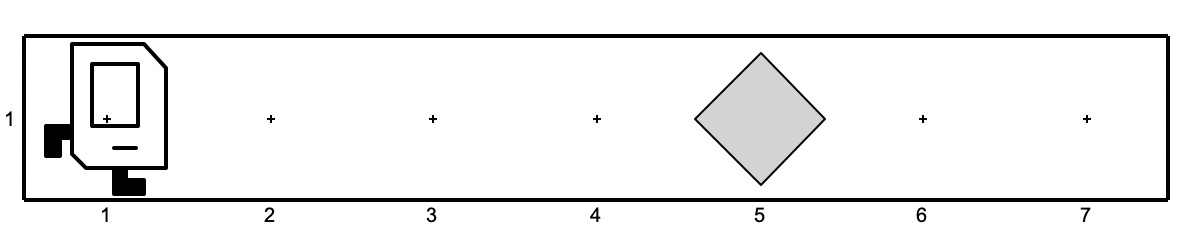
\includegraphics[scale=\figscale]{images/ch02/gpb/init.jpg}
        \caption{မူလ အနေအထား}    
    \end{subfigure}
    \begin{subfigure}[t]{{\figpctw}\textwidth}
        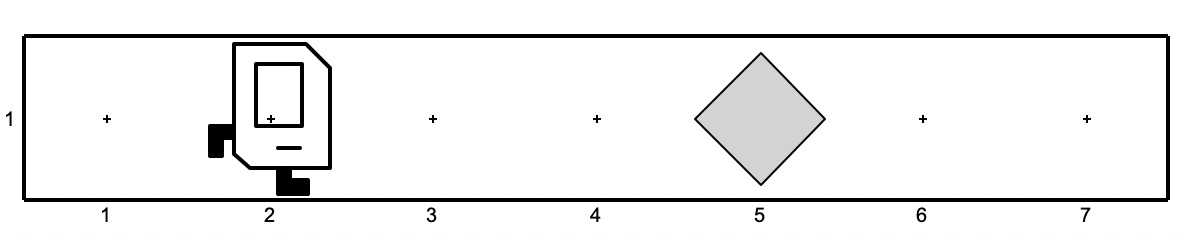
\includegraphics[scale=\figscale]{images/ch02/gpb/1st_iter.jpg}
        \caption{ပထမ တစ်ကျော့ပြီး}    
    \end{subfigure}
    \begin{subfigure}[t]{{\figpctw}\textwidth}
        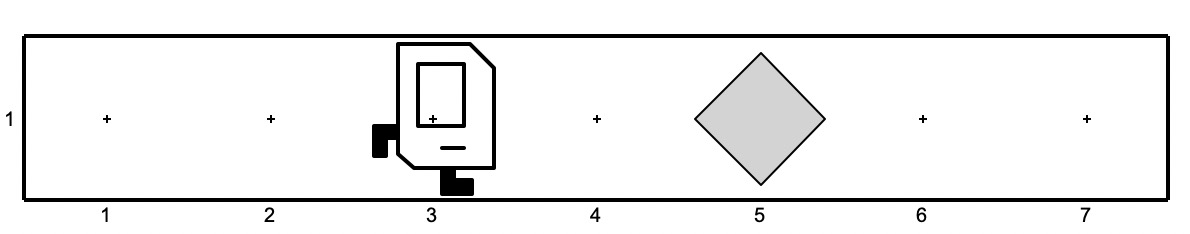
\includegraphics[scale=\figscale]{images/ch02/gpb/2nd_iter.jpg}
        \caption{ဒုတိယ တစ်ကျော့ပြီး}    
    \end{subfigure}
    \begin{subfigure}[t]{{\figpctw}\textwidth}
        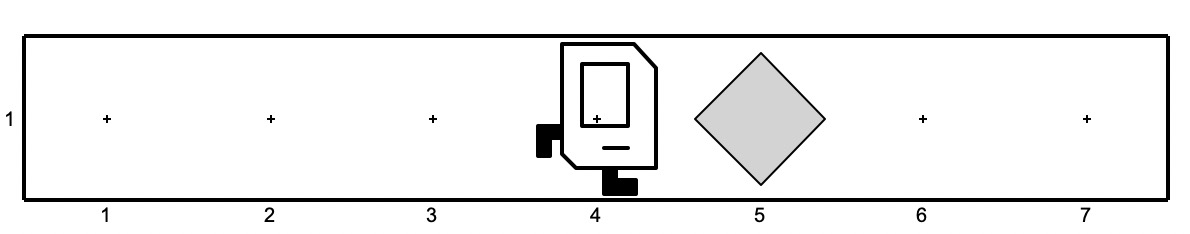
\includegraphics[scale=\figscale]{images/ch02/gpb/3rd_iter.jpg}
        \caption{တတိယ တစ်ကျော့ပြီး}    
    \end{subfigure}
    \begin{subfigure}[t]{{\figpctw}\textwidth}
        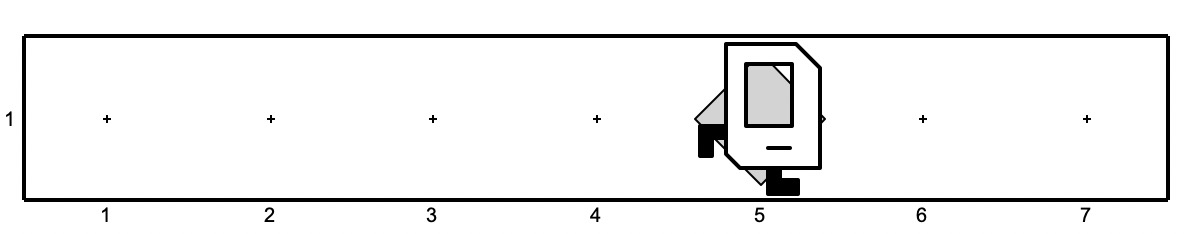
\includegraphics[scale=\figscale]{images/ch02/gpb/4th_iter.jpg}
        \caption{စတုတ္ထမြောက် ကျော့ပြီး}    
    \end{subfigure}   
    \caption{}
    \label{fig:gpb_iters}
\end{figure}


အပြည့်အစုံ ဖော်ပြပေးထားတဲ့ ပရိုဂရမ်ကို လေ့လာကြည့်ပါ။

%
\setlength{\fboxsep}{0pt}
\begin{minted}[frame=\mintframe, framerule=\mintrule,framesep= \mintsep, xleftmargin=\xlftmargin
    , bgcolor=mintbgcolor,rulecolor=mintrulecolor
    , python3=true,escapeinside=ßß]{python}
# File: go_pick_beeper.py
from stanfordkarel import *


def main():
    while no_beepers_present():
        move()

    pick_beeper()


if __name__ == "__main__":
    run_karel_program("go_pick_beeper")

\end{minted}
%

\subsection*{ကားရဲလ် ကွန်ဒီရှင်များ}
\fCode{beepers\_present} ကွန်ဒီရှင် ကျတော့ လက်ရှိကွန်နာမှာ ဘိပါရှိရင် အမှန်၊ မရှိရင် အမှား ရလဒ်ထွက်တယ်။ \fCode{no\_beep\allowbreak ers\_present} နဲ့ ဆန့်ကျင်ဘက်ပေါ့။ ကားရဲလ် ကွန်ဒီရှင်တွေအားလုံးကို တေဘဲလ် (\fRefNo{\ref{tbl:karel_conditions}}) မှာ  ကြည့်ပါ။ ပုံမှန်စစ်တာနဲ့ အငြင်းပုံစံစစ်တာ နှစ်မျိုးကို ယှဉ်တွဲပြထားပါတယ်။
%
\begin{flushleft}
\vspace{1em}
\setlength{\extrarowheight}{3pt}
\begin{tabular}[h]{*{3}l}
    \toprule[1.5pt]
        \fTblHead{ကွန်ဒီရှင်} & \fTblHead{ဆန့်ကျင်ဘက် ကွန်ဒီရှင်} & \fTblHead{စစ်ပေးသည့် အခြေအနေ}\\       
    \midrule
    \fCode{front\_is\_clear} & \fCode{front\_is\_blocked} & \fMMSm{ရှေ့မှာ နံရံကပ်လျက် ရှိမရှိ}\\
    \fCode{left\_is\_clear} & \fCode{left\_is\_blocked} & \fMMSm{ဘယ်ဘက်မှာ နံရံကပ်လျက် ရှိမရှိ}\\
    \fCode{right\_is\_clear} & \fCode{right\_is\_blocked} & \fMMSm{ညာဘက်မှာ နံရံကပ်လျက် ရှိမရှိ}\\
    \fCode{beepers\_present} & \fCode{no\_beepers\_present} & \fMMSm{လက်ရှိကွန်နာမှာ ဘိပါရှိမရှိ}\\
    \fCode{beepers\_in\_bag} & \fCode{no\_beepers\_in\_bag} & \fMMSm{ကားရဲလ်၏ ဘိပါအိပ်ထဲ  ဘိပါရှိမရှိ}\\   
    \fCode{facing\_north} & \fCode{not\_facing\_north} & \fMMSm{အရှေ့ဘက် မျက်နှာမူလျက် ရှိမရှိ}\\
    \fCode{facing\_east} & \fCode{not\_facing\_east} & \fMMSm{အနောက်ဘက် မျက်နှာမူလျက် ရှိမရှိ}\\
    \fCode{facing\_west} & \fCode{not\_facing\_west} & \fMMSm{တောင်ဘက် မျက်နှာမူလျက် ရှိမရှိ}\\
    \fCode{facing\_south} & \fCode{not\_facing\_south} & \fMMSm{မြောက်ဘက် မျက်နှာမူလျက် ရှိမရှိ}\\   
    \bottomrule[1.5pt]
\end{tabular}
\label{tbl:karel_conditions}
\captionof{table}{ကားရဲလ် စစ်နိုင်သည့် ကွန်ဒီရှင်များ}
\end{flushleft}
%

\subsection*{\fSubSecCodeBf{while} loop ဆင်းတက်စ်}
\fCode{while} \fEn{loop} ရေးတဲ့ ပုံစံက ယေဘုယျအားဖြင့် ဒီလိုပါ။ 
%
\setlength{\fboxsep}{0pt}
\begin{minted}[frame=\mintframe, framerule=\mintrule,framesep= \mintsep, xleftmargin=\xlftmargin
    , bgcolor=mintbgcolor,rulecolor=mintrulecolor
    , python3=true,escapeinside=ßß]{python}
while ß$condition$ß :
    ß$statement_1$ß
    ß$statement_2$ß
    ß$statement_3$ \fEn{etc.}ß
\end{minted}
%
\fEnEmp{condition} က ကားရဲလ်ကွန်ဒီရှင် တစ်ခုဖြစ်တယ်။ ကော်လံ \fCode{:} မကျန်ခဲ့အောင် ဂရုစိုက်ပါ။ \fEnEmp{condition} မှန်နေသေးသ၍ ပြန်ကျော့စေချင်တဲ့ စတိတ်မန့်တွေကို \fCode{while} အောက်မှာ အင်ဒန့်ထ်လုပ်ထား ရပါမယ်။ ရှေ့မှာရှင်းနေသ၍ \fCode{move} လုပ်တဲ့ \fCode{while} \fEn{loop} ကို အခုလို
%
\setlength{\fboxsep}{0pt}
\begin{minted}[frame=\mintframe, framerule=\mintrule,framesep= \mintsep, xleftmargin=\xlftmargin
    , bgcolor=mintbgcolor,rulecolor=mintrulecolor
    , python3=true,escapeinside=ßß]{python}
while front_is_clear():
    move()
\end{minted}
%
ရေးပါတယ်။

\subsection*{‘Make Beeper Row’ ဥပမာ}
\fEn{‘Make Row of Five Beepers’} ဥပမာမှာ လမ်းရဲ့အလျားဟာ မပြောင်းလဲဘူး ယူဆတာမို့လို့  \fCode{for} \fEn{loop} ကို အသုံးပြုတာ ဆီလျော်ပါတယ်။ လမ်းရဲ့အရှည်ကို ကြိုမသိထားဘူး၊ တစ်လမ်းလုံး ဘိပါတွေ ဖြန့်ထားပေးရမယ်ဆိုရင် \fCode{while} နဲ့ ရေးရမှာပါ။
%
\setlength{\fboxsep}{0pt}
\begin{minted}[frame=\mintframe, framerule=\mintrule,framesep= \mintsep, xleftmargin=\xlftmargin
    , bgcolor=mintbgcolor,rulecolor=mintrulecolor
    , python3=true,escapeinside=ßß]{python}
# File: make_beeper_row.py
from stanfordkarel import *


def main():
    while front_is_clear():
        put_beeper()
        move()

    put_beeper()


if __name__ == "__main__":
    run_karel_program()

\end{minted}
%

တစ်ကြိမ်ကျော့ပြီးတိုင်း  ရှိနေမဲ့ အနေအထားကို ပုံ (\fRefNo{\ref{fig:mbr_iters}}) မှာ ကြည့်ပါ။ လေးကြိမ်မြောက်အပြီး \fCode{front\_is\_clear} စစ်တဲ့အခါ မှားနေပြီဖြစ်လို့ ထပ်မကျော့တော့ဘဲ \fEn{loop} ကနေ ထွက်သွားမယ်။ ဒီအခါမှာ ဘိပါတစ်ခု လိုနေသေးတယ်။ \fCode{put\_beeper} ထပ်လုပ်ရမယ်။ တစ်ခါပဲ လုပ်ရမှာပါ။ ဒါကြောင့် \fCode{while} \fEn{loop} ထဲမပါအောင် ပထမအဆင့် အင်ဒန့်ထ်ပဲ ဖြစ်ရမယ်။ 


\begin{figure}[tbh!]
    \newcommand{\figpctw}{0.455}
    \newcommand{\figscale}{0.16}
    \begin{subfigure}[t]{{\figpctw}\textwidth}
        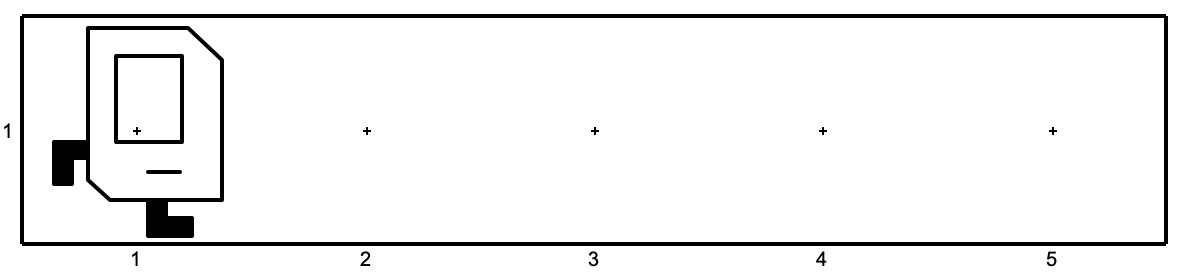
\includegraphics[scale=\figscale]{images/ch02/mbr/init.jpg}
        \caption{မူလ အနေအထား}    
    \end{subfigure}
    \begin{subfigure}[t]{{\figpctw}\textwidth}
        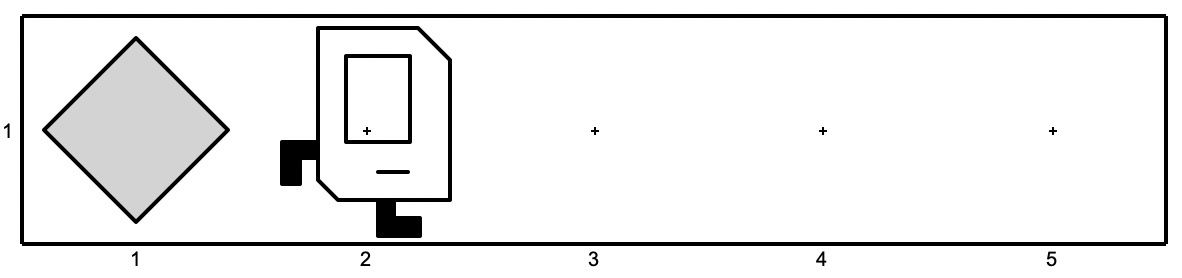
\includegraphics[scale=\figscale]{images/ch02/mbr/1st_iter.jpg}
        \caption{ပထမ တစ်ကျော့ပြီး}    
    \end{subfigure}
    \begin{subfigure}[t]{{\figpctw}\textwidth}
        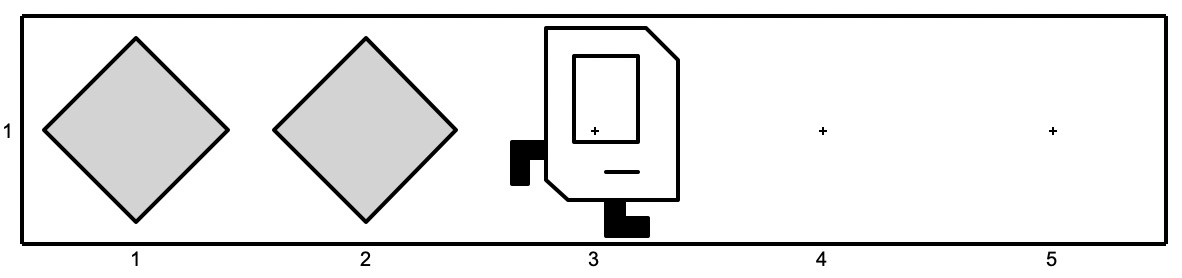
\includegraphics[scale=\figscale]{images/ch02/mbr/2nd_iter.jpg}
        \caption{ဒုတိယ တစ်ကျော့ပြီး}    
    \end{subfigure}
    \begin{subfigure}[t]{{\figpctw}\textwidth}
        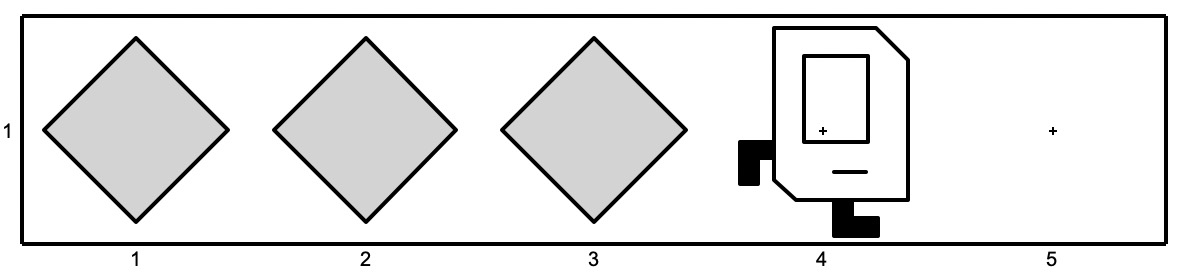
\includegraphics[scale=\figscale]{images/ch02/mbr/3rd_iter.jpg}
        \caption{တတိယ တစ်ကျော့ပြီး}    
    \end{subfigure}
    \begin{subfigure}[t]{{\figpctw}\textwidth}
        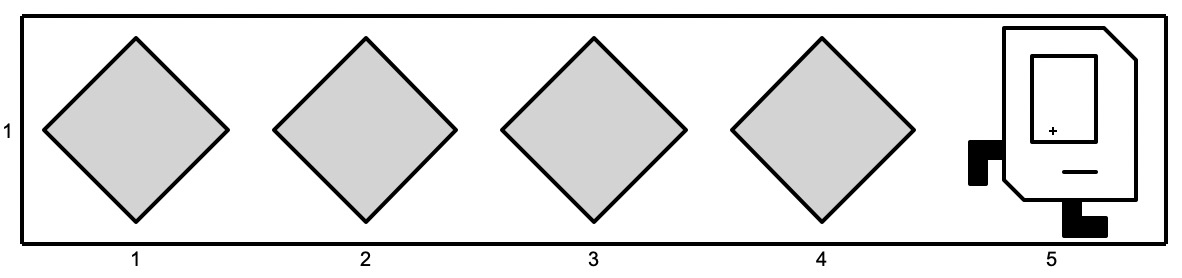
\includegraphics[scale=\figscale]{images/ch02/mbr/4th_iter.jpg}
        \caption{စတုတ္ထမြောက် ကျော့ပြီး}    
    \end{subfigure}   
    \caption{}
    \label{fig:mbr_iters}
\end{figure}

\section{\fSecCodeBf{if} စတိတ်မန့်}
တစ်ခု (သို့) တစ်ခုထက်ပိုတဲ့ စတိတ်မန့်တွေကို အခြေအနေတစ်ရပ် မှန်တော့မှပဲ လုပ်ဆောင်စေချင်တဲ့အခါ \fCodeBf{if} ကို အသုံးပြုနိုင်တယ်။ ဥပမာ
%
\setlength{\fboxsep}{0pt}
\begin{minted}[frame=\mintframe, framerule=\mintrule,framesep= \mintsep, xleftmargin=\xlftmargin
    , bgcolor=mintbgcolor,rulecolor=mintrulecolor
    , python3=true,escapeinside=ßß]{python}
if beepers_present():
    pick_beeper()
\end{minted}
%
\fCode{if} စတိတ်မန့်ဟာ \fCode{beepers\_present} ကွန်ဒီရှင် မှန်တော့မှပဲ \fCode{pick\_beeper} လုပ်မှာပါ။ မှားရင် မလုပ်ပါဘူး။

ပုံမှာတွေ့ရတဲ့ ကမ္ဘာနှစ်ခုထဲက တစ်ခုမှာ ကားရဲလ်ရှိနေမယ် ဆိုပါစို့။
%
\begin{figure}[tbh!]
    \newcommand{\figpctw}{0.5}
    \newcommand{\figscale}{0.14}
    \begin{subfigure}[t]{{\figpctw}\textwidth}
        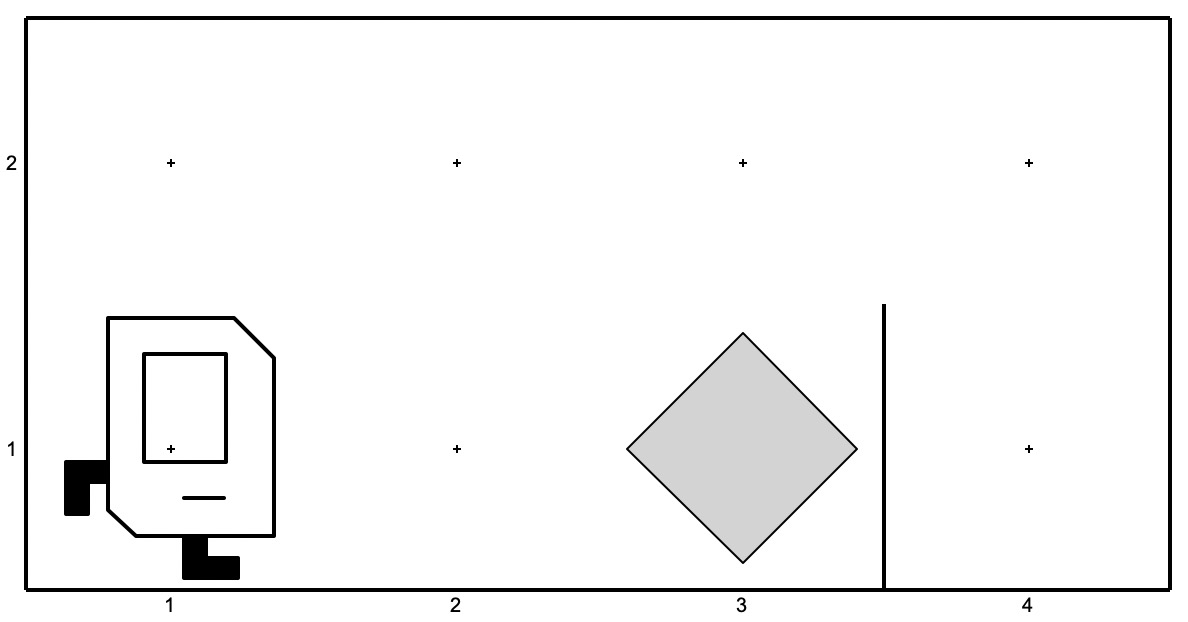
\includegraphics[scale=\figscale]{images/ch02/move_beeper_to_other_side_if_any/init1.jpg}
        \caption{}     
    \end{subfigure}
    \begin{subfigure}[t]{{\figpctw}\textwidth}
        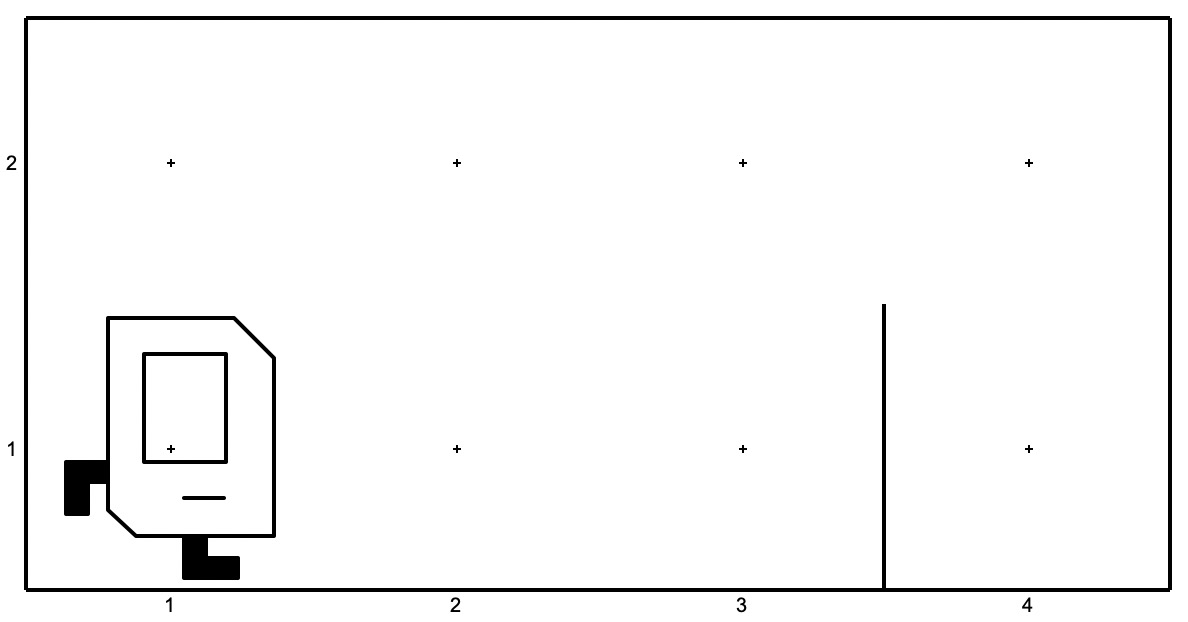
\includegraphics[scale=\figscale]{images/ch02/move_beeper_to_other_side_if_any/init2.jpg}
        \caption{}    
    \end{subfigure}  
    \caption{}
    \label{fig:mbtos_if_any}
\end{figure}
%
ဘိပါရှိတဲ့ ကမ္ဘာဆိုရင် ဘိပါကို နံရံအခြားဘက် အောက်ခြေကို ရွှေ့ပေးရမယ်။ မရှိတဲ့ကမ္ဘာဆိုရင် နံရံ ဒီဘက် အောက်ခြေမှာပဲ ရပ်နေရမယ်။ ပရိုဂရမ်က ကမ္ဘာနှစ်ခုလုံးမှာ မှန်အောင် အလုပ် လုပ်နိုင်ရပါမယ်။ ဒီအတွက် \fCode{if} စတိတ်မန့် သုံးထားတာ လေ့လာကြည့်ပါ။ 
%
\setlength{\fboxsep}{0pt}
\begin{minted}[frame=\mintframe, framerule=\mintrule,framesep= \mintsep, xleftmargin=\xlftmargin
    , bgcolor=mintbgcolor,rulecolor=mintrulecolor
    , python3=true,escapeinside=ßß]{python}
# File: move_beeper_to_other_side_if_any.py
from stanfordkarel import *


def main():
    move()
    move()
    if beepers_present():
        pick_beeper()
        turn_left()
        move()
        # turn_right
        turn_left()
        turn_left()
        turn_left()
        move()
        # turn_right
        turn_left()
        turn_left()
        turn_left()
        move()
        put_beeper()
        turn_left()


if __name__ == "__main__":
    run_karel_program("mbtos1")

\end{minted}
%
\fCode{if} အောက်က စတိတ်မန့်တွေကို အင်ဒန့်ထ်လုပ်ထားတာ သတိပြုပါ။ အဲဒီ စတိတ်မန့်အားလုံး \fCode{beepers\_\allowbreak present} ဖြစ်မှ လုပ်ဆောင်မှာ ဖြစ်တယ်။ ဘိပါမရှိတဲ့ ကမ္ဘာမှာ စမ်းကြည့်ဖို့အတွက် \mytcboxinl{\fEnSnd{Load World}} ခလုတ်နှိပ်ပြီး ခေါ်တင်ပါ။  ဒါမှမဟုတ် ပရိုဂရမ်ကုဒ်မှာ \fCode{"mbtos2"} လို့ပြင်ပြီး ပြန် \fEn{run} ပါ။  

\fCode{if} စတိတ်မန့် ယေဘုယျစထရက်ချာကို အခုလိုတွေ့ရတယ်။
%
\setlength{\fboxsep}{0pt}
\begin{minted}[frame=\mintframe, framerule=\mintrule,framesep= \mintsep, xleftmargin=\xlftmargin
    , bgcolor=mintbgcolor,rulecolor=mintrulecolor
    , python3=true,escapeinside=ßß]{python}
if ß$condition$ß :
    ß$statement_1$ß
    ß$statement_2$ß
    ß$statement_3$ \fEn{etc.}ß
\end{minted}
%
\fEnEmp{condition} က \fCode{front\_is\_clear}\fEn{,} \fCode{beepers\_present} စတဲ့ ကားရဲလ် ကွန်ဒီရှင် တစ်ခုခုဖြစ်မယ်။ တေဘဲလ် (\fRefNo{\ref{tbl:karel_conditions}}) မှာ ကားရဲလ်ကို စစ်ခိုင်းလို့ရတဲ့ ကွန်ဒီရှင်အားလုံး ပြထားပါတယ်။


\section{\fSecCodeBf{if...else} စတိတ်မန့်}
အခြေအနေတစ်ရပ် မှန်တဲ့အခါ လုပ်ဆောင်ရမှာနဲ့ မှားတဲ့အခါ လုပ်ဆောင်ရမှာ မတူကွဲပြားနေတဲ့အခါ \fCodeBf{if}\fCode{...}\fCodeBf{else} ကို သုံးပါတယ်။ ရှေ့က \fCode{if} စတိတ်မန့် ဥပမာ ပုံ (\fRefNo{\ref{fig:mbtos_if_any}})  မှာ ဘိပါမရှိရင် နဂိုမူလနေရာကို ပြန်လာခိုင်းချင်တယ်ဆိုပါစို့။ \fCode{if...else} နဲ့ အခုလို ရေးရပါမယ်။
%
\setlength{\fboxsep}{0pt}
\begin{minted}[frame=\mintframe, framerule=\mintrule,framesep= \mintsep, xleftmargin=\xlftmargin
    , bgcolor=mintbgcolor,rulecolor=mintrulecolor
    , python3=true,escapeinside=ßß]{python}
from stanfordkarel import *


def main():
    move()
    move()
    if beepers_present():
        pick_beeper()
        turn_left()
        move()
        # turn_right
        turn_left()
        turn_left()
        turn_left()
        move()
        # turn_right
        turn_left()
        turn_left()
        turn_left()
        move()
        put_beeper()
        turn_left()
    else:
        turn_left()
        turn_left()
        move()
        move()
        turn_left()
        turn_left()


if __name__ == "__main__":
    run_karel_program("mbtos2")
\end{minted}
%

\fCode{if...else} စတိတ်မန့်က ကွန်ဒီရှင်မှန်ရင်  \fCode{if} ဘလောက်ကိုလုပ်ဆောင်ပေးပြီး ကွန်ဒီရှင်မှားရင်တော့ \fCode{else} ဘလောက်ကို လုပ်ဆောင်ပေးတာပါ။ ယေဘုယျပုံစံက ဒီလိုပါ
%
\setlength{\fboxsep}{0pt}
\begin{minted}[frame=\mintframe, framerule=\mintrule,framesep= \mintsep, xleftmargin=\xlftmargin
    , bgcolor=mintbgcolor,rulecolor=mintrulecolor
    , python3=true,escapeinside=ßß]{python}
if ß$condition$ß :
    ß$statement_{1a}$ß
    ß$statement_{2a}$ß
    ß$statement_{3a}$ \fEn{etc.}ß
else:
    ß$statement_{1b}$ß
    ß$statement_{2b}$ß
    ß$statement_{3b}$ \fEn{etc.}ß
\end{minted}
%

\section{Nested ကွန်ထရိုးလ် စတိတ်မန့်များ}
% ===============
ကွန်ထရိုးလ် စတိတ်မန့် ဘလောက်ထဲမှာ ကွန်ထရိုးလ် စတိတ်မန့် ရှိလို့ရတယ်။။ \fEn{Nested} ကွန်ထရိုးလ် စတိတ်မန့်လို့ ခေါ်ပါတယ်။ 

\subsection*{Nested \fSubSecCodeBf{for} loop}
%
\setlength{\fboxsep}{0pt}
\begin{minted}[frame=\mintframe, framerule=\mintrule,framesep= \mintsep, xleftmargin=\xlftmargin
    , bgcolor=mintbgcolor,rulecolor=mintrulecolor
    , python3=true,escapeinside=ßß]{python}
for i in range(4):
    for j in range(3):
        put_beeper()
    move()
\end{minted}
%
အခုလို \fCode{for} \fEn{loop} နှစ်ခု ဆင့်ရေးထားတာကို \fEn{nested} \fCode{for} \fEn{loop} လို့ခေါ်ပါတယ်။ ပထမ \fCode{for} ဘလောက်ထဲမှာ နောက်ထပ် \fCode{for} \fEn{loop} တစ်ခု ပါဝင်နေတာပါ။ \fEn{Loop} တစ်ခုချင်းကို သီးခြား ရည်ညွှန်းချင်တဲ့အခါ အပြင် \fCode{for} \fEn{loop} နဲ့ အတွင်း \fCode{for} \fEn{loop} လို့ ပြောလေ့ရှိတယ်။ အပြင် \fCode{for} \fEn{loop} မှာ ဗေရီရေဘဲလ် \fCode{i} ဆိုရင် အတွင်းမှာ \fCode{i} မဖြစ်ရပါဘူး။ \fCode{j}\fEn{,} ဒါမှမဟုတ် \fCode{k} မတူတာ  တစ်ခုခုဖြစ်ရပါမယ်။ 

အပြင် \fCode{for} \fEn{loop} ဘလောက်ထဲမှာ အတွင်း \fCode{for} \fEn{loop} နဲ့ \fCode{move} ပါဝင်တယ်။ အတွင်း \fCode{for} \fEn{loop} က  \fCode{put\_beeper} သုံးကြိမ်ကျော့ထားတာ ဖြစ်တဲ့အတွက် အဲဒီ အပြင် \fCode{for} \fEn{loop} ဘလောက်ဟာ အောက်ပါအတိုင်း \fCode{put\_beeper} သုံးကြိမ်လုပ်ပြီး \fCode{move} လုပ်တာနဲ့ တူတယ်လို့ မြင်နိုင်တယ်။ 
%
\setlength{\fboxsep}{0pt}
\begin{minted}[frame=\mintframe, framerule=\mintrule,framesep= \mintsep, xleftmargin=\xlftmargin
    , bgcolor=mintbgcolor,rulecolor=mintrulecolor
    , python3=true,escapeinside=ßß]{python}
for i in range(4):
    put_beeper()
    put_beeper()
    put_beeper()
    move()
\end{minted}
%
%
\setlength{\fboxsep}{0pt}
\begin{minted}[frame=\mintframe, framerule=\mintrule,framesep= \mintsep, xleftmargin=\xlftmargin
    , bgcolor=mintbgcolor,rulecolor=mintrulecolor
    , python3=true,escapeinside=ßß]{python}
for i in range(4):
    for j in range(3):
        put_beeper()
    move()
\end{minted}
%

အတန်းလိုက် ကွန်နာ ငါးခုမှာ တစ်ကွန်နာ ဘိပါ (၂၅) ခုစီ ချထားပေးဖို့  \fEn{nested loop} နဲ့ ရေးထားတာကို လေ့လာကြည့်ပါ။
%
\setlength{\fboxsep}{0pt}
\begin{minted}[frame=\mintframe, framerule=\mintrule,framesep= \mintsep, xleftmargin=\xlftmargin
    , bgcolor=mintbgcolor,rulecolor=mintrulecolor
    , python3=true,escapeinside=ßß]{python}
# File: row_of_beeper_piles.py
from stanfordkarel import *


def main():
    for i in range(4):
        for j in range(25):
            put_beeper()
        move()

    for i in range(25):
        put_beeper()


if __name__ == "__main__":
    run_karel_program("5x1")
\end{minted}
%

\subsection*{Nested \fSubSecCodeBf{for} and \fSubSecCodeBf{while}}
ကမ္ဘာပါတ်လည် ဘိပါခြံစည်းရိုး ခတ်ပေးဖို့အတွက် \fCode{for} နဲ့ \fCode{while} \fEn{nest} လုပ်ထားတာကို လေ့လာကြည့်ပါ။ (၁, ၁) ကွန်နာမှာ အရှေ့ဘက်လည့် အနေအထားကနေ စမယ်လို့ ယူဆပါ။ ကမ္ဘာအရွယ်အစား အမျိုးမျိုးကို ခြံစည်းရိုး ခတ်ပေးနိုင်ရပါမယ်။

တောင်ဘက် နံရံတလျှောက် ဘိပါတွေချသွားမယ် (နောက်ဆုံး ကွန်နာမှာ ဘိပါမချဘဲ ချန်ထားမယ်)။ ပြီးရင် အရှေ့ဘက် နံရံအတွက် အဆင်သင့်ဖြစ်အောင် ဘယ်ဘက်လှည့်မယ်။ ပုံ (\fRefNo{\ref{fig:beeper_fence_iters}}) (က) နဲ့ (ခ) ကို ကြည့်ပါ။ အရှေ့၊ မြောက် နဲ့ အနောက်ဘက် နံရံတွေအတွက်လည်း ဒီအတိုင်း လုပ်သွားရုံပါပဲ။ ပုံ (\fRefNo{\ref{fig:beeper_fence_iters}}) (ဂ)၊ (ဃ)၊ (င) အသီးသီးကို ကြည့်ပါ။

နံရံတစ်ဘက် အတွက် ဆိုရင် အခုလို
%
\setlength{\fboxsep}{0pt}
\begin{minted}[frame=\mintframe, framerule=\mintrule,framesep= \mintsep, xleftmargin=\xlftmargin
    , bgcolor=mintbgcolor,rulecolor=mintrulecolor
    , python3=true,escapeinside=ßß]{python}
while front_is_clear():
    put_beeper()
    move()
turn_left()
\end{minted}
%
ဖြစ်မယ်။ (\fCode{while} ဘလောက်မှာ  \fCode{turn\_left} မပါတာ ဂရုပြုပါ)။ နံရံလေးဘက်အတွက် လေးကြိမ် လုပ်ရမှာဆိုတော့ \fCode{for} နဲ့ အခုလို
%
\setlength{\fboxsep}{0pt}
\begin{minted}[frame=\mintframe, framerule=\mintrule,framesep= \mintsep, xleftmargin=\xlftmargin
    , bgcolor=mintbgcolor,rulecolor=mintrulecolor
    , python3=true,escapeinside=ßß]{python}
# File: beeper_fence.py
for i in range(4):
    while front_is_clear():
        put_beeper()
        move()
    turn_left()
\end{minted}
%
ရေးရပါမယ်။

\begin{figure}[tbh!]
    \newcommand{\figpctw}{0.3}
    \newcommand{\figscale}{0.1}
    \begin{subfigure}[t]{{\figpctw}\textwidth}
        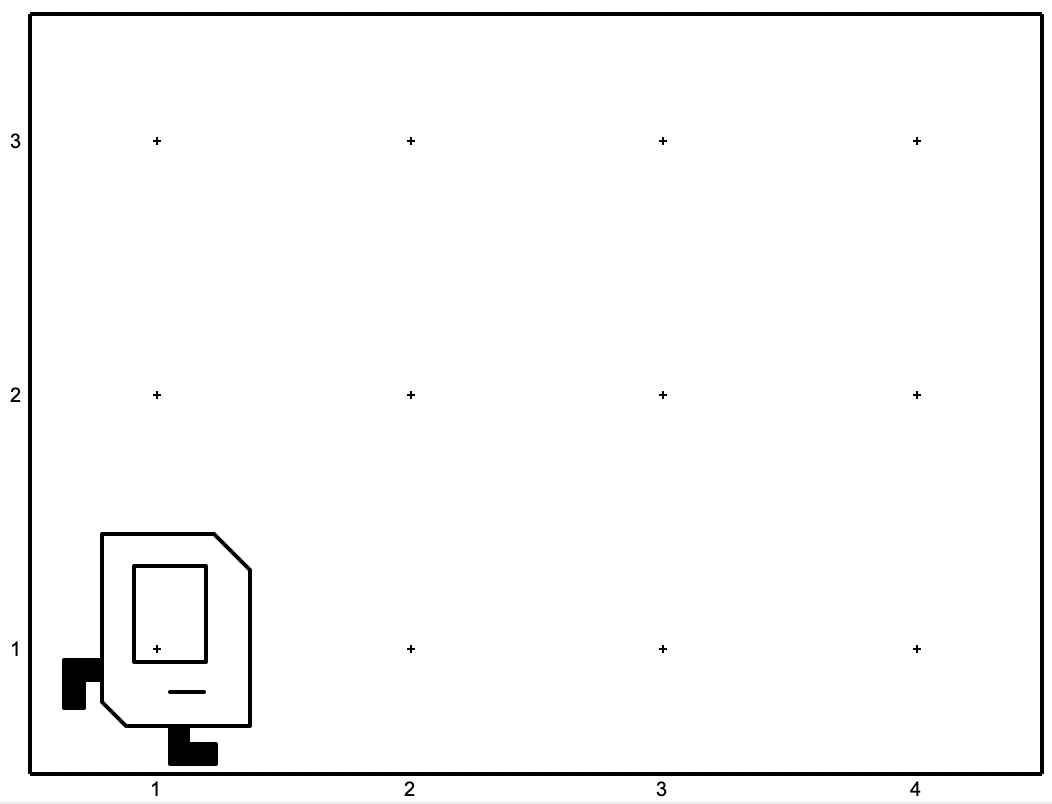
\includegraphics[scale=\figscale]{images/ch02/beeper_fence/init.jpg}
        \caption{မူလ အနေအထား}    
    \end{subfigure}
    \begin{subfigure}[t]{{\figpctw}\textwidth}
        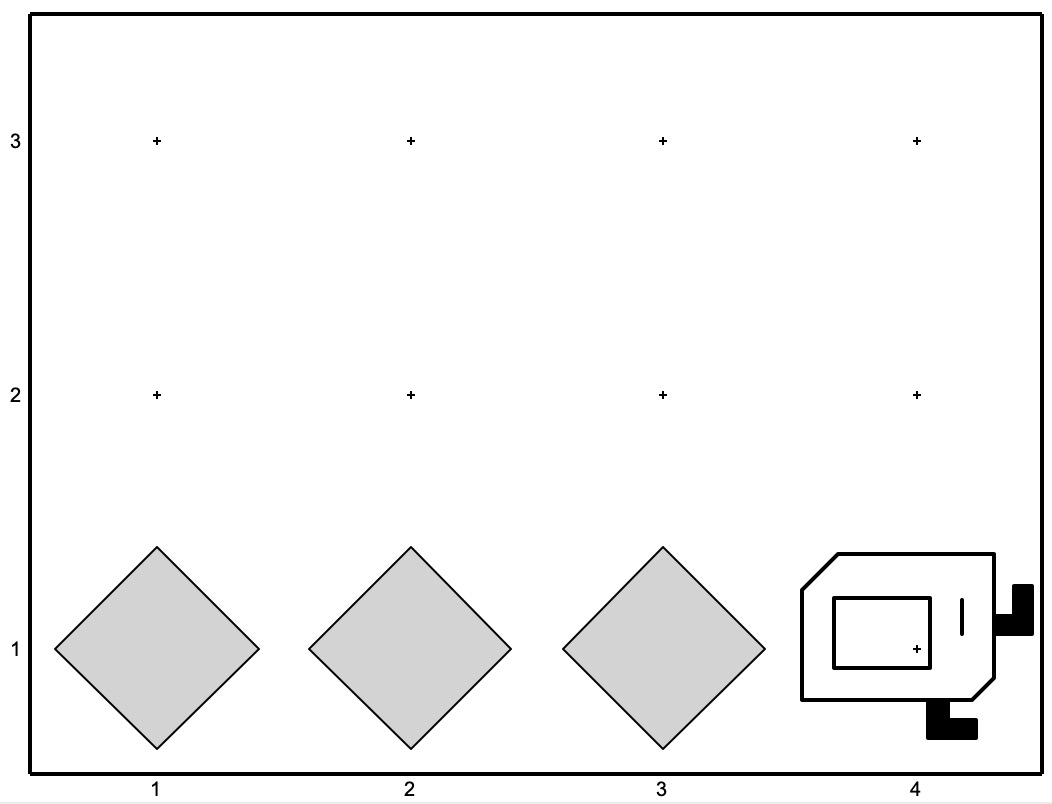
\includegraphics[scale=\figscale]{images/ch02/beeper_fence/1st_iter.jpg}
        \caption{ပထမ တစ်ကျော့ပြီး}    
    \end{subfigure}
    \begin{subfigure}[t]{{\figpctw}\textwidth}
        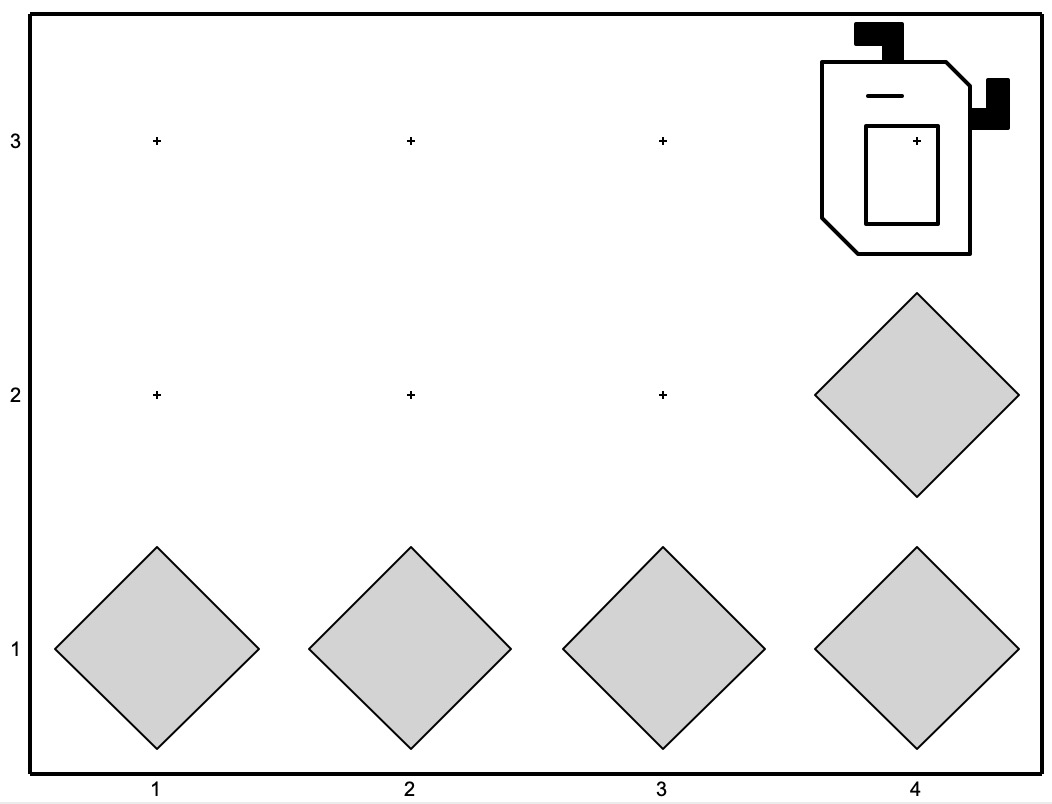
\includegraphics[scale=\figscale]{images/ch02/beeper_fence/2nd_iter.jpg}
        \caption{ဒုတိယ တစ်ကျော့ပြီး}    
    \end{subfigure}
    \begin{subfigure}[t]{{\figpctw}\textwidth}
        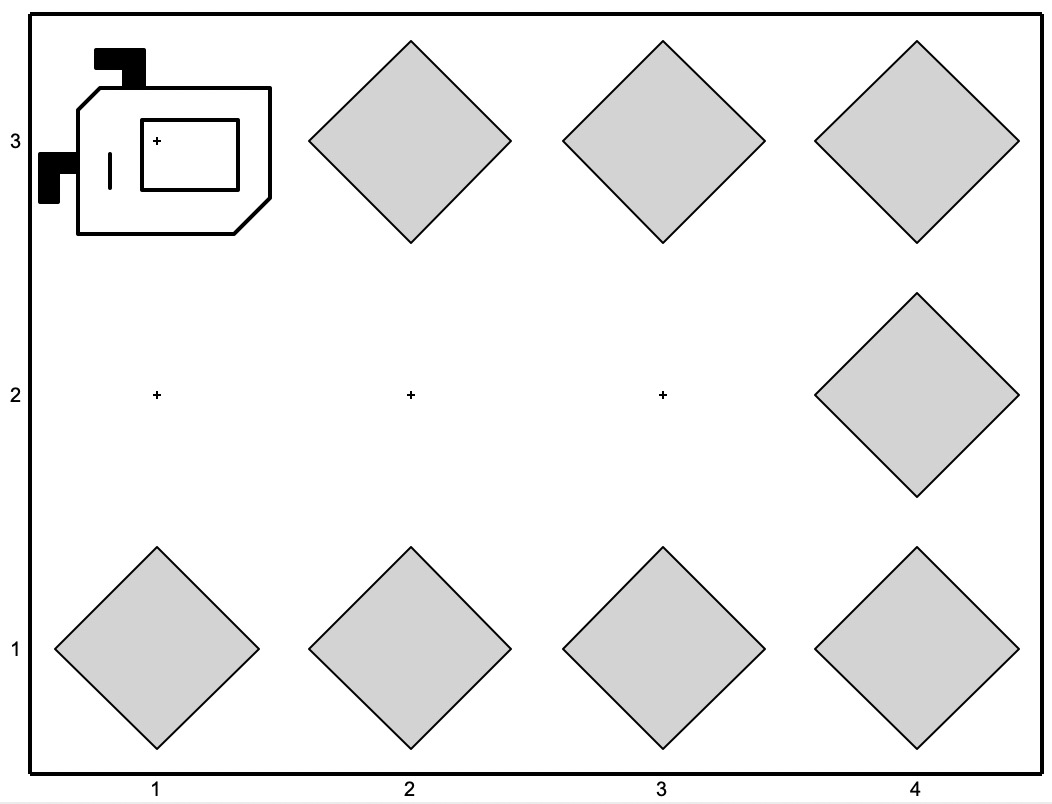
\includegraphics[scale=\figscale]{images/ch02/beeper_fence/3rd_iter.jpg}
        \caption{တတိယ တစ်ကျော့ပြီး}    
    \end{subfigure}
    \begin{subfigure}[t]{{\figpctw}\textwidth}
        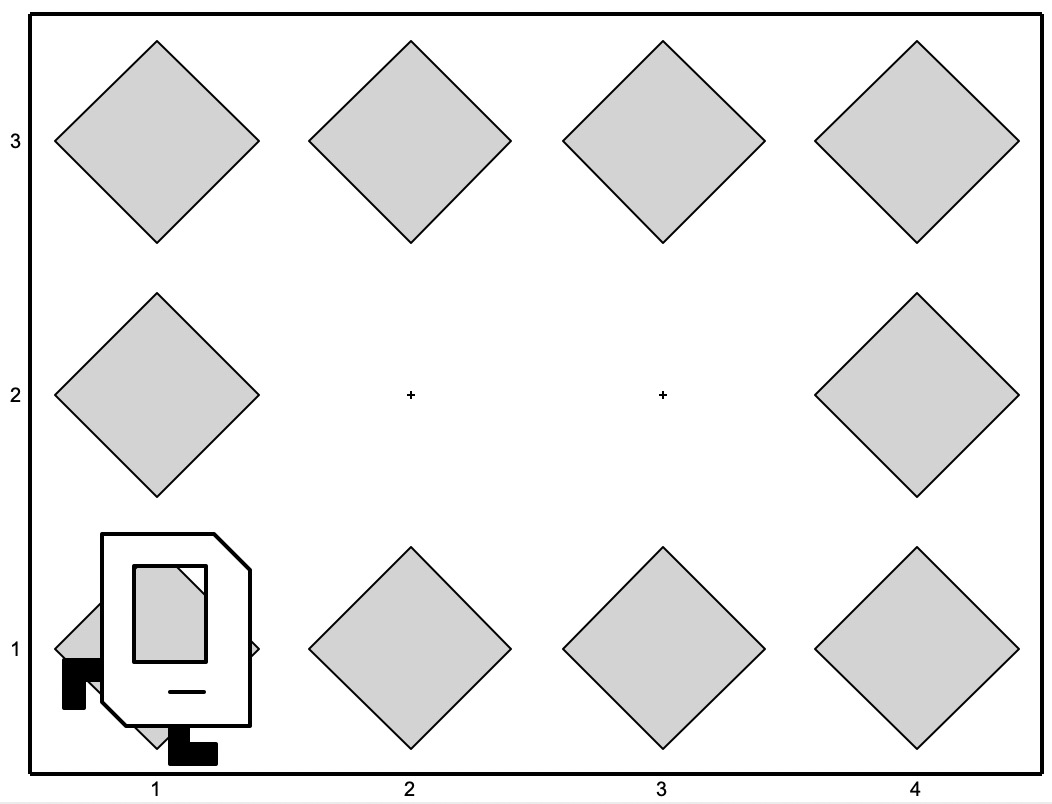
\includegraphics[scale=\figscale]{images/ch02/beeper_fence/4th_iter.jpg}
        \caption{စတုတ္ထမြောက် ကျော့ပြီး}    
    \end{subfigure}   
    \caption{}
    \label{fig:beeper_fence_iters}
\end{figure}

ပရိုဂရမ် တစ်ခုလုံး အတွက်ဆိုရင် အခုလိုပါ
%
\setlength{\fboxsep}{0pt}
\begin{minted}[frame=\mintframe, framerule=\mintrule,framesep= \mintsep, xleftmargin=\xlftmargin
    , bgcolor=mintbgcolor,rulecolor=mintrulecolor
    , python3=true,escapeinside=ßß]{python}
# File: beeper_fence.py
from stanfordkarel import *


def main():
    for i in range(4):
        while front_is_clear():
            put_beeper()
            move()
        turn_left()


if __name__ == "__main__":
    run_karel_program("4x3")

\end{minted}
%

\subsection*{Nested \fSubSecCodeBf{while} and \fSubSecCodeBf{if}}
\fCode{while} နဲ့ \fCode{if} \fEn{nest} လုပ်လို့လည်း ရတာပေါ့။ လမ်းပေါ်မှာ ဘိပါတွေက ကြုံရာကျပန်း  ရှိနေမယ်။ ဘိပါတွေကို အမှိုက်တွေလို့ ယူဆပြီး ရှင်းပေးရပါမယ်။ လမ်းအလျားကို ကြိုမသိဘူး၊ ကွန်နာတစ်ခုမှာ ဘိပါတစ်ခုထက် ပိုမရှိနိုင်ဘူးလို့ ယူဆပါ။  လမ်းအဆုံးထိ \fCode{while} \fEn{loop} နဲ့ ရွှေ့ခိုင်းလို့ ရမယ်။ ရောက်တဲ့ ကွန်နာတိုင်းမှာ ဘိပါရှိရင် ကောက်ခိုင်းရပါမယ်။ \fCode{if} သုံးရမယ်။
%
\setlength{\fboxsep}{0pt}
\begin{minted}[frame=\mintframe, framerule=\mintrule,framesep= \mintsep, xleftmargin=\xlftmargin
    , bgcolor=mintbgcolor,rulecolor=mintrulecolor
    , python3=true,escapeinside=ßß]{python}
from stanfordkarel import *


def main():
    while front_is_clear():
        if beepers_present():
            pick_beeper()
        move()

    if beepers_present():
        pick_beeper()


if __name__ == "__main__":
    run_karel_program("clean_the_street")

\end{minted}
%
\fCode{if} စတိတ်မန့် နဲ့ \fCode{move} ကို \fCode{while} \fEn{loop} ရဲ့ ဘလောက်ထဲမှာ ထည့်ပြီး ရှေ့မှာရှင်းနေသ၍ ပြန်ကျော့ခိုင်းထားတာပါ။ \fCode{if} စတိတ်မန့်က ဘိပါရှိတော့မှပဲ ကောက်ပေးဖို့အတွက်။

ပြီးခဲ့တဲ့ဟာနဲ့ အလားတူတဲ့ နောက်ထပ် ဥပမာ တစ်ခုကတော့ လမ်းတစ်လျှောက် ကွန်နာတွေမှာ ဘိပါရှိရင် ကောက်ခိုင်းပြီး မရှိရင် တစ်ခုချပေးရပါမယ်။ တနည်းအားဖြင့် ကွန်နာတစ်ခုချင်းရဲ့ ဘိပါရှိ/မရှိ အခြေအနေကို ဆန့်ကျင်ဘက် ပြောင်းတာပေါ့။
%
\setlength{\fboxsep}{0pt}
\begin{minted}[frame=\mintframe, framerule=\mintrule,framesep= \mintsep, xleftmargin=\xlftmargin
    , bgcolor=mintbgcolor,rulecolor=mintrulecolor
    , python3=true,escapeinside=ßß]{python}
# File: toggle_beepers.py
from stanfordkarel import *


def main():
    while front_is_clear():
        if beepers_present():
            pick_beeper()
        else:
            put_beeper()
        move()

    if beepers_present():
        pick_beeper()


if __name__ == "__main__":
    run_karel_program("toggle_beepers")
\end{minted}
%
\fCode{if...else} သုံးထားတယ်။ ကျန်တာအားလုံး လမ်းရှင်းတဲ့ ပရိုဂရမ်နဲ့ တူတူပဲ။


\subsection*{Nested \fSubSecCodeBf{if}}
အခြေအနေ တစ်ရပ် မှန်တော့မှပဲ လုပ်ချင်ရင် \fCode{if} ကို သုံးတယ်။  
အခြေအနေ ‘နှစ်ရပ်’ လုံးနဲ့ ကိုက်ညီမှ လုပ်ဆောင်စေချင်တဲ့အခါ \fEn{nested} \fCode{if} သုံးနိုင်ပါတယ်။ ညာဘက်လည်းရှင်း လက်ရှိကွန်နာမှာလည်း ဘိပါမရှိမှ ဘိပါတစ်ခု ချထားခိုင်းမယ်ဆိုပါစို့။ အခုလိုရေးနိုင်ပါတယ်
%
\setlength{\fboxsep}{0pt}
\begin{minted}[frame=\mintframe, framerule=\mintrule,framesep= \mintsep, xleftmargin=\xlftmargin
    , bgcolor=mintbgcolor,rulecolor=mintrulecolor
    , python3=true,escapeinside=ßß]{python}
if right_is_clear():
    if no_beepers_present():
        put_beeper()
\end{minted}
%
ညာဘက်မှာ ရှင်းနေမှ အပြင် \fCode{if} က အတွင်း \fCode{if} ကို လုပ်ဆောင်စေမှာပါ။ အတွင်း \fCode{if} ကလည်း ဘိပါမရှိမှပဲ \fCode{put\_beeper} လုပ်မှာပါ။ ညာဘက်မှာ ပိတ်နေရင်သော်လည်းကောင်း ဘိပါရှိနေရင်သော်လည်းကောင်း \fCode{pick\_beeper} လုပ်မှာ မဟုတ်ပါဘူး။ \fCode{right\_is\_clear} နဲ့ \fCode{no\_beepers\_present} အခြေအနေ နှစ်ခုလုံး မှန်မှပဲ လုပ်မှာပါ။

ပုံ (\fRefNo{\ref{fig:st_repair}}) (က) မှာ ဒုတိယ လမ်းတစ်လျှောက် လမ်းပြင်တဲ့အလုပ်ကို ကားရဲလ်ကို တာဝန်ပေးတယ်လို့ ယူဆပါ။ ဘိပါရော ညာဘက်နံရံပါ မရှိတဲ့ ကွန်နာတွေက  လမ်းအခြေအနေ တော်တော်ဆိုးနေတဲ့ နေရာတွေ။ ဒီလိုနေရာတွေမှာ ဘိပါတစ်ခု ဖြည့်ပြီး လမ်းပြင်ပေးရမှာပါ။ 
%
\setlength{\fboxsep}{0pt}
\begin{minted}[frame=\mintframe, framerule=\mintrule,framesep= \mintsep, xleftmargin=\xlftmargin
    , bgcolor=mintbgcolor,rulecolor=mintrulecolor
    , python3=true,escapeinside=ßß]{python}
# File: repair_street.py
from stanfordkarel import *


def main():
    while front_is_clear():
        if right_is_clear():
            if no_beepers_present():
                put_beeper()
        move()

    if right_is_clear():
        if no_beepers_present():
            put_beeper()


if __name__ == "__main__":
    run_karel_program("repair_street")
\end{minted}
%
\fCode{while} ဘလောက်ထဲမှာ \fEn{nested} \fCode{if} နဲ့ \fCode{move} ပါဝင်တယ်။ \fEn{nested} \fCode{if} က ညာဘက်လည်းရှင်း ဘိပါလည်းမရှိမှ လက်ရှိကွန်နာမှာ ဘိပါတစ်ခု ချခိုင်းထားတာပါ။  \fCode{while} ထဲမှာ \fCode{if}၊ အဲဒီ \fCode{if} ထဲမှာမှ နောက်ထပ် \fCode{if} တစ်ခု ဆင့်ထားတဲ့အတွက် သုံးဆင့် \fEn{nest} လုပ်ထားတာပါ။ အင်ဒန့်ထ် လုပ်ထားတာတွေ ဂရုစိုက်ကြည့်ဖို့ လိုတယ်။ ဘယ်ဘလောက်ထဲမှာ ဘာရှိနေလဲဆိုတာ မြင်အောင် လုပ်ရမှာပါ။ ကိုယ်တိုင်ရေးရင်လည်း အင်ဒန့်ထ် ဂရုစိုက်ပြီး လုပ်ရပါမယ်။ လမ်းပြင်ပြီး အခြေအနေကို ညာဘက် ပုံ (\fRefNo{\ref{fig:st_repair}}) (ခ) တွင် ကြည့်ပါ။

\begin{figure}[tbh!]
    \newcommand{\figpctw}{0.48}
    \newcommand{\figscale}{0.15}
    \begin{subfigure}[t]{{\figpctw}\textwidth}
        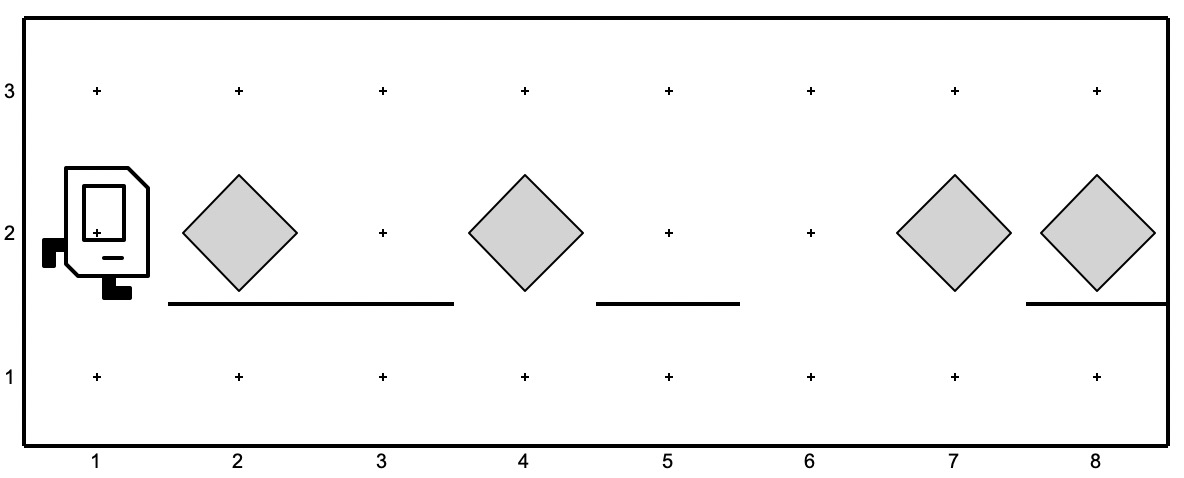
\includegraphics[scale=\figscale]{images/ch02/st_repair/init.jpg}
        \caption{မူလ အနေအထား}    
    \end{subfigure}
    \begin{subfigure}[t]{{\figpctw}\textwidth}
        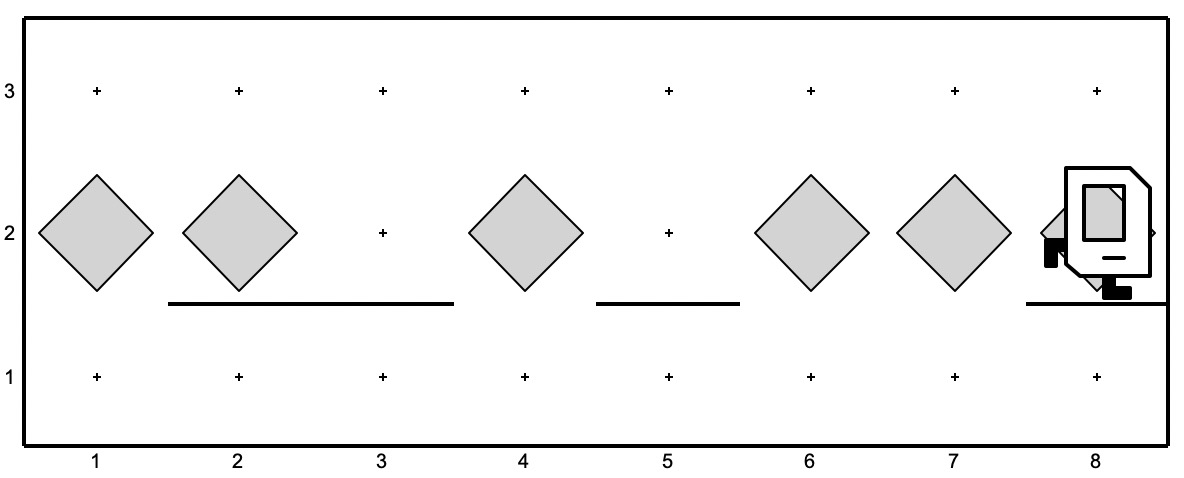
\includegraphics[scale=\figscale]{images/ch02/st_repair/after.jpg}
        \caption{လမ်းပြင်ပြီး အနေအထား}    
    \end{subfigure}
    \caption{}
    \label{fig:st_repair}
\end{figure}



% keyords in text
        
%Italic
%    Indicates new terms, URLs, email addresses, filenames, and file extensions.
%Constant width
%    Used for program listings, as well as within paragraphs to refer to program elements such as variable or function %names, databases, data types, environment variables, statements, and keywords.
%
%    Note that when a line break falls within a constant_width term, a hyphen is not added—it could be misunderstood as %part of the term.
%Constant width bold
%Shows commands or other text that should be typed literally by the user.
%    Constant width italic
%    Shows text that should be replaced with user-supplied values or by values determined by context.